\documentclass[border=1cm]{standalone}

\usepackage{tikz}

\usetikzlibrary{shapes, arrows, calc, positioning}
\definecolor{codegreen}{rgb}{0, 0.6, 0}
\definecolor{codegray}{rgb}{0.5, 0.5, 0.5}
\definecolor{codepurple}{rgb}{0.58, 0, 0.82}
\definecolor{backcolour}{rgb}{0.95, 0.95, 0.92}

\tikzstyle{decision} = [diamond, draw, fill=blue!20, text width=4.5em, text badly centered, node distance=3cm, inner sep=0pt]
\tikzstyle{block} = [rectangle, draw, fill=blue!20, text centered, rounded corners, minimum height=2em]
\tikzstyle{line} = [draw, -latex']
\tikzstyle{cloud} = [draw, ellipse, fill=red!20, node distance=5em, minimum height=2em]
\tikzset
{
    -|-/.style=
    {
        to path=
        {
            (\tikztostart) -| ($(\tikztostart)!#1!(\tikztotarget)$) |- (\tikztotarget)
            \tikztonodes
        }
    },
    -|-/.default=0.5,
    |-|/.style=
    {
        to path=
        {
            (\tikztostart) |- ($(\tikztostart)!#1!(\tikztotarget)$) -| (\tikztotarget)
            \tikztonodes
        }
    },
    |-|/.default=0.5,
}

\begin{document}
    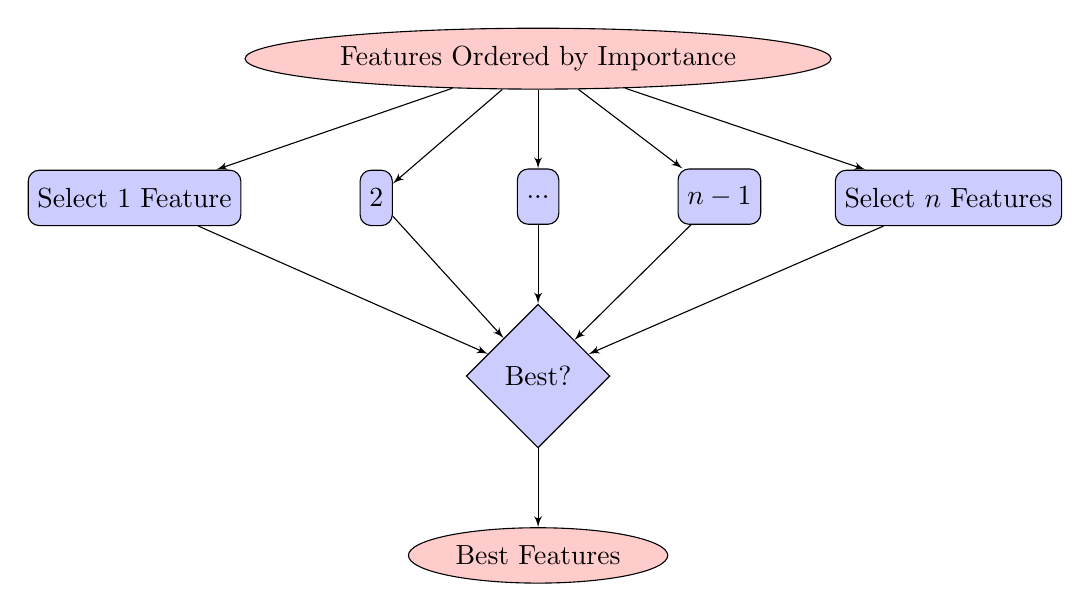
\begin{tikzpicture}
        \node[cloud] (00) {Features Ordered by Importance};

        \node[block, below left=1.6cm of 00] (01) {Select 1 Feature};
        \path[line] (00) -- (01);

        \node[block, right=1.5cm of 01] (02) {2};
        \path[line] (00) -- (02);

        \node[block, below=1cm of 00] (03) {...};
        \path[line] (00) -- (03);

        \node[block, right=1.5cm of 03] (04) {$n-1$};
        \path[line] (00) -- (04);

        \node[block, below right=1.6cm of 00] (05) {Select $n$ Features};
        \path[line] (00) -- (05);

        \node[decision, below=1cm of 03] (06) {Best?};
        \path[line] (01) -- (06);
        \path[line] (02) -- (06);
        \path[line] (03) -- (06);
        \path[line] (04) -- (06);
        \path[line] (05) -- (06);

        \node[cloud, below=1cm of 06] (07) {Best Features};
        \path[line] (06) -- (07);
    \end{tikzpicture}
\end{document}